\begin{tiny}(Ccp42)\end{tiny} L'ensemble est formé par les points de trois demi-droites (figure \ref{fig:Ccp42_1}). L'ensemble des affixes étant
\begin{displaymath}
 \left] -\infty, 2\right[ 
 \cup
 \left\lbrace \lambda e^{\frac{2i\pi}{3}}, \lambda \in \left] -\infty, 2\right[\right\rbrace 
 \cup
 \left\lbrace \lambda e^{\frac{-2i\pi}{3}}, \lambda \in  \left] -\infty, 2\right[\right\rbrace 
\end{displaymath}
\begin{figure}
 \centering
 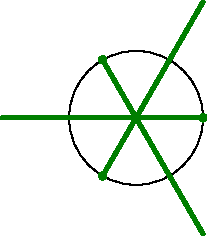
\includegraphics{./Ccp42_1.pdf}
 \caption{Exercice \theenumi \hspace{0.2cm}\tiny{(Ccp42)}}
 \label{fig:Ccp42_1}
\end{figure}
